% !TeX root = ../summary-syssec.tex

\section{Intel SGX (Software Guard Extension)}
\subsection{Basics}
\begin{itemize}
  \item Security enhancements in Intel CPUs
  \item Enclave = security-critical part of the application
  \item Main goal:
    \begin{itemize}
      \item Enable secure execution in otherwise untrusted platforms (OS, ...)
      \item Enclave data confidentiality and execution integrity
    \end{itemize}
  \item Idea: Reduce TCB and trust boundary.
    \begin{center}
      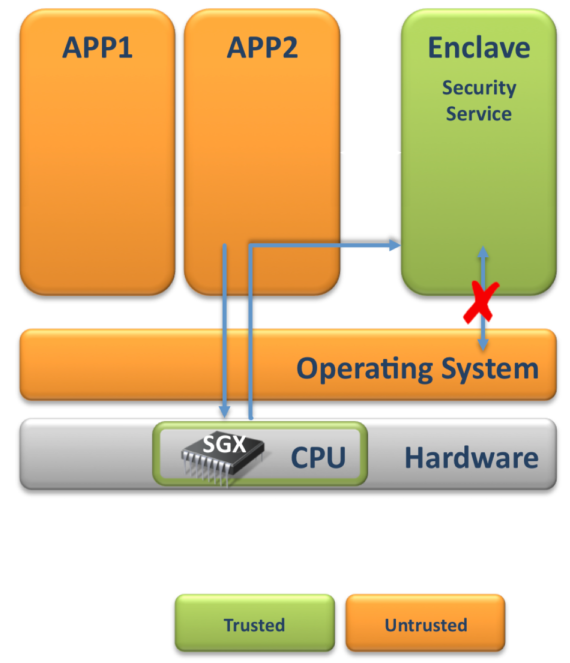
\includegraphics[width=0.3\columnwidth]{sgx_idea.png}
    \end{center}
  \item Trusted are:
    \begin{itemize}
      \item Intel
      \item The CPU
      \item Quoting Enclave
      \item Intel SGX Trusted Libraries
    \end{itemize}
  \item Not trusted:
    \begin{itemize}
      \item BIOS, Firmware
      \item OS
      \item Other software running on the machine
      \item Other hardware (e.g. memory, motherboard)
    \end{itemize}
  \item Unique set of keys are burned into the processor.
  \item Parallel Execution of different Enclaves possible.
\end{itemize}

\subsection{Enclave Creation}
\begin{center}
  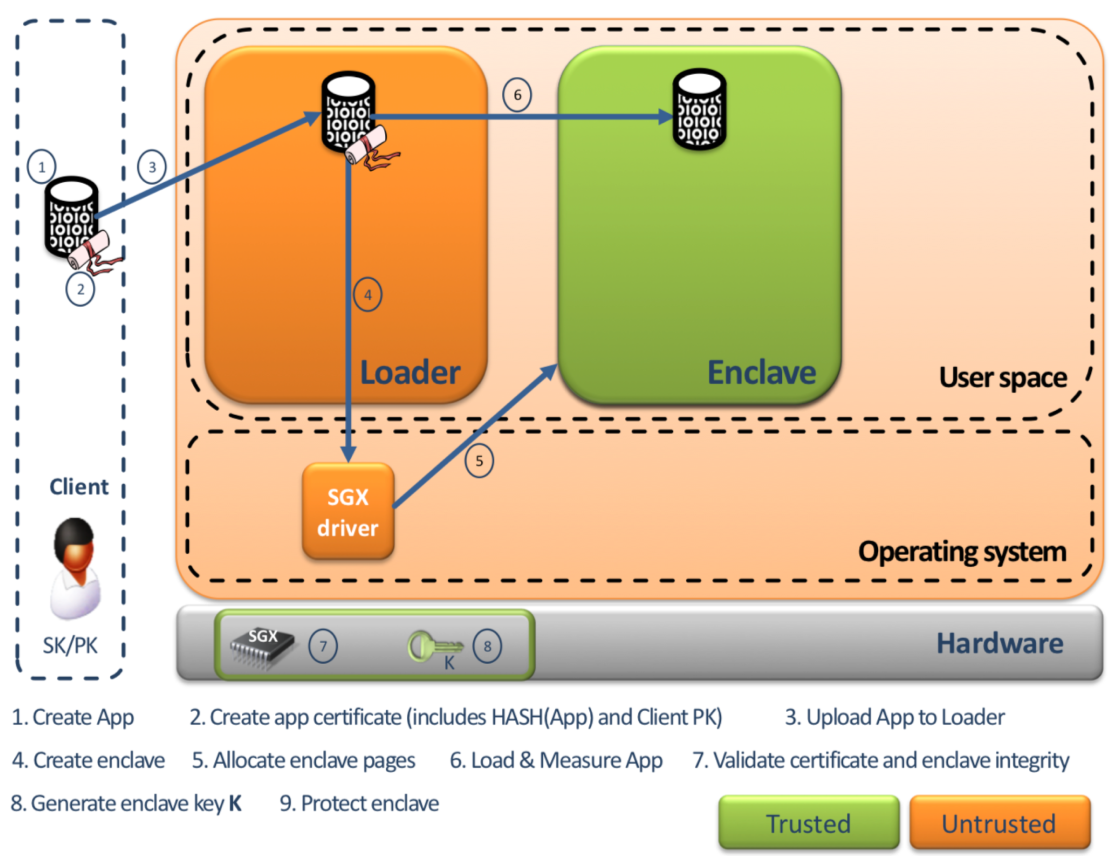
\includegraphics[width=0.9\columnwidth]{sgx_create_enclave.png}
\end{center}

\subsection{Sealing}
\begin{itemize}
  \item Store encrypted confidential data on disk. Only Enclave can access it.
  \item Enclave has no direct access to IO / storage.
  \item Same Enclave ID on the same platform can unseal it's sealed data.
  \item Enclave will loose state across reboots, but can unseal it's sealed
    state.
\end{itemize}


\subsection{Attestation and secure communication}
\begin{itemize}
  \item Two enclaves can communicate securely over an untrusted channel.
  \item Remote Attestation allows Enclave to check whether other instance is a
    valid and secure SGX Enclave:
    \begin{enumerate}
      \item Verifier sends nonce.
      \item Enclave generates report.
      \item Pass report to quoting enclave which verifies the report.
      \item Signs report with the platform key and send to the verifier.
    \end{enumerate}
\end{itemize}

\subsection{Application: DelegaTEE}
\begin{itemize}
  \item Owner's credentials remain confidential.
  \item The Owner can restrict access to his account (in time, actions,
    ...)
  \item Difficult to distinguish between access by the
    Delegatee and Owner
  \item Functioning:
    \begin{center}
      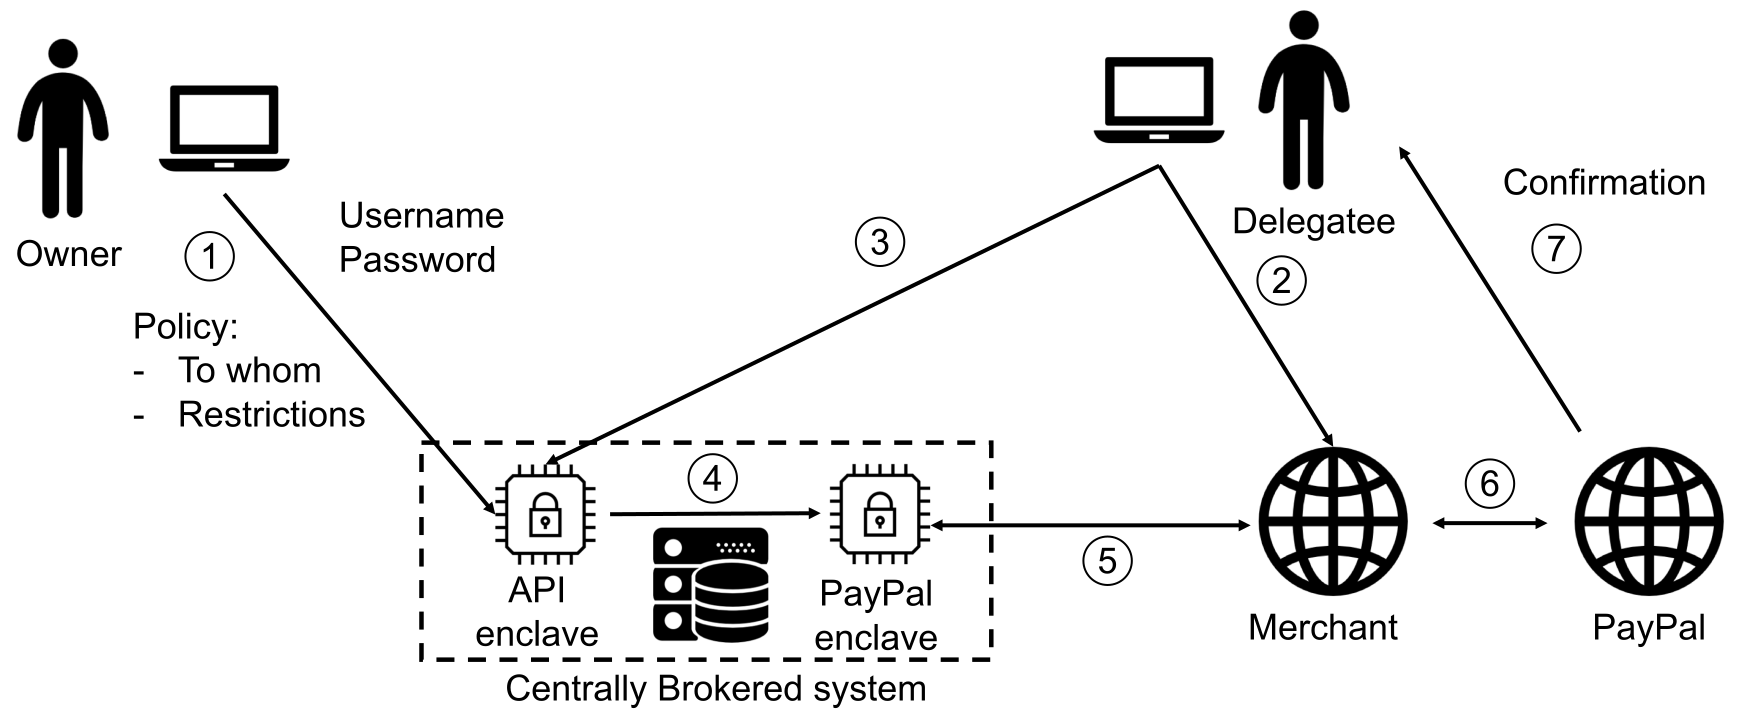
\includegraphics[width=0.9\columnwidth]{sgx_delegatee.png}
    \end{center}
  \item Applications: Email access, website access, e-banking, paypal
  \item May undermine service (e.g. Netflix) and create market for sharing
    economy
  \item Two systems possible: centrally brokered or decentralized
    peer-to-peer
\end{itemize}

\subsection{Attacks}
\subsubsection{Cache-timing attack}
\begin{itemize}
  \item  PMC
    \begin{itemize}
      \item Use Performance Monitoring Counters (PMC) to count cache misses
	(instead of timing L1 vs. L2)
      \item Enabled by privileged adversary
    \end{itemize}
  \item  isolate victim
    \begin{itemize}
      \item Assign the attack process and victim enclave to separate core
      \item Reduces noise
    \end{itemize}
  \item  hyper-threading
    \begin{itemize}
      \item Run uninterrupted victim enclave and attacker in parallel
      \item Complicates attack detection
    \end{itemize}
  \item Attack target
    \begin{itemize}
      \item Attack non-cryptographic computations
    \end{itemize}
\end{itemize}
Generic and efficient defenses  are an open problem.

\subsubsection{Page Fault Attack}
Page faults allow the OS to observe input-dependent control transfer or
input-dependent data access. Thereby the OS can infer the execution flow and
can observe otherwise protected inputs.

Protection: Rewrite s.t. memory access pattern does not depend on input.
